\PassOptionsToPackage{unicode=true}{hyperref} % options for packages loaded elsewhere
\PassOptionsToPackage{hyphens}{url}
%
\documentclass[a4paper,11pt]{memoir}
%\documentclass[]{article}
\usepackage{lmodern}
\usepackage{amssymb,amsmath}
\usepackage{ifxetex,ifluatex}
\usepackage{fixltx2e} % provides \textsubscript
\ifnum 0\ifxetex 1\fi\ifluatex 1\fi=0 % if pdftex
  \usepackage[T1]{fontenc}
  \usepackage[utf8]{inputenc}
  \usepackage{textcomp} % provides euro and other symbols
\else % if luatex or xelatex
  \usepackage{unicode-math}
  \defaultfontfeatures{Ligatures=TeX,Scale=MatchLowercase}
\fi
% use upquote if available, for straight quotes in verbatim environments
\IfFileExists{upquote.sty}{\usepackage{upquote}}{}
% use microtype if available
\IfFileExists{microtype.sty}{%
\usepackage[]{microtype}
\UseMicrotypeSet[protrusion]{basicmath} % disable protrusion for tt fonts
}{}
\IfFileExists{parskip.sty}{%
\usepackage{parskip}
}{% else
\setlength{\parindent}{0pt}
\setlength{\parskip}{6pt plus 2pt minus 1pt}
}
\usepackage{hyperref}
\hypersetup{
            pdftitle={Datasets in "sdam" package},
            pdfauthor={Antonio Rivero Ostoic},
            pdfborder={0 0 0},
            breaklinks=true}
\urlstyle{same}  % don't use monospace font for urls
\usepackage[left=2cm,right=2cm,top=2cm,bottom=2cm]{geometry}
\usepackage{color}
\usepackage{fancyvrb}
\newcommand{\VerbBar}{|}
\newcommand{\VERB}{\Verb[commandchars=\\\{\}]}
\DefineVerbatimEnvironment{Highlighting}{Verbatim}{commandchars=\\\{\}}
% Add ',fontsize=\small' for more characters per line
\usepackage{framed}
\definecolor{shadecolor}{RGB}{248,248,248}
\newenvironment{Shaded}{\begin{snugshade}}{\end{snugshade}}
\newcommand{\AlertTok}[1]{\textcolor[rgb]{0.94,0.16,0.16}{#1}}
\newcommand{\AnnotationTok}[1]{\textcolor[rgb]{0.56,0.35,0.01}{\textbf{\textit{#1}}}}
\newcommand{\AttributeTok}[1]{\textcolor[rgb]{0.77,0.63,0.00}{#1}}
\newcommand{\BaseNTok}[1]{\textcolor[rgb]{0.00,0.00,0.81}{#1}}
\newcommand{\BuiltInTok}[1]{#1}
\newcommand{\CharTok}[1]{\textcolor[rgb]{0.31,0.60,0.02}{#1}}
\newcommand{\CommentTok}[1]{\textcolor[rgb]{0.56,0.35,0.01}{\textit{#1}}}
\newcommand{\CommentVarTok}[1]{\textcolor[rgb]{0.56,0.35,0.01}{\textbf{\textit{#1}}}}
\newcommand{\ConstantTok}[1]{\textcolor[rgb]{0.00,0.00,0.00}{#1}}
\newcommand{\ControlFlowTok}[1]{\textcolor[rgb]{0.13,0.29,0.53}{\textbf{#1}}}
\newcommand{\DataTypeTok}[1]{\textcolor[rgb]{0.13,0.29,0.53}{#1}}
\newcommand{\DecValTok}[1]{\textcolor[rgb]{0.00,0.00,0.81}{#1}}
\newcommand{\DocumentationTok}[1]{\textcolor[rgb]{0.56,0.35,0.01}{\textbf{\textit{#1}}}}
\newcommand{\ErrorTok}[1]{\textcolor[rgb]{0.64,0.00,0.00}{\textbf{#1}}}
\newcommand{\ExtensionTok}[1]{#1}
\newcommand{\FloatTok}[1]{\textcolor[rgb]{0.00,0.00,0.81}{#1}}
\newcommand{\FunctionTok}[1]{\textcolor[rgb]{0.00,0.00,0.00}{#1}}
\newcommand{\ImportTok}[1]{#1}
\newcommand{\InformationTok}[1]{\textcolor[rgb]{0.56,0.35,0.01}{\textbf{\textit{#1}}}}
\newcommand{\KeywordTok}[1]{\textcolor[rgb]{0.13,0.29,0.53}{\textbf{#1}}}
\newcommand{\NormalTok}[1]{#1}
\newcommand{\OperatorTok}[1]{\textcolor[rgb]{0.81,0.36,0.00}{\textbf{#1}}}
\newcommand{\OtherTok}[1]{\textcolor[rgb]{0.56,0.35,0.01}{#1}}
\newcommand{\PreprocessorTok}[1]{\textcolor[rgb]{0.56,0.35,0.01}{\textit{#1}}}
\newcommand{\RegionMarkerTok}[1]{#1}
\newcommand{\SpecialCharTok}[1]{\textcolor[rgb]{0.00,0.00,0.00}{#1}}
\newcommand{\SpecialStringTok}[1]{\textcolor[rgb]{0.31,0.60,0.02}{#1}}
\newcommand{\StringTok}[1]{\textcolor[rgb]{0.31,0.60,0.02}{#1}}
\newcommand{\VariableTok}[1]{\textcolor[rgb]{0.00,0.00,0.00}{#1}}
\newcommand{\VerbatimStringTok}[1]{\textcolor[rgb]{0.31,0.60,0.02}{#1}}
\newcommand{\WarningTok}[1]{\textcolor[rgb]{0.56,0.35,0.01}{\textbf{\textit{#1}}}}
\usepackage{graphicx,grffile}
\makeatletter
\def\maxwidth{\ifdim\Gin@nat@width>\linewidth\linewidth\else\Gin@nat@width\fi}
\def\maxheight{\ifdim\Gin@nat@height>\textheight\textheight\else\Gin@nat@height\fi}
\makeatother
% Scale images if necessary, so that they will not overflow the page
% margins by default, and it is still possible to overwrite the defaults
% using explicit options in \includegraphics[width, height, ...]{}
\setkeys{Gin}{width=\maxwidth,height=\maxheight,keepaspectratio}
\setlength{\emergencystretch}{3em}  % prevent overfull lines
\providecommand{\tightlist}{%
  \setlength{\itemsep}{0pt}\setlength{\parskip}{0pt}}
\setcounter{secnumdepth}{0}
% Redefines (sub)paragraphs to behave more like sections
\ifx\paragraph\undefined\else
\let\oldparagraph\paragraph
\renewcommand{\paragraph}[1]{\oldparagraph{#1}\mbox{}}
\fi
\ifx\subparagraph\undefined\else
\let\oldsubparagraph\subparagraph
\renewcommand{\subparagraph}[1]{\oldsubparagraph{#1}\mbox{}}
\fi

% set default figure placement to htbp
\makeatletter
\def\fps@figure{htbp}
\makeatother

\usepackage{hyperref}
\PassOptionsToPackage{bookmarks=false}{hyperref}

\makeatletter
\renewcommand{\figurename}{Fig.}
\renewcommand{\thefigure}{\@arabic\c@figure}
\makeatother


\title{Datasets in \texttt{"sdam"} package}
\author{Antonio Rivero Ostoic}
\date{September 2022}

\begin{document}
\maketitle

\hypertarget{preliminaries}{%
\subsection{Preliminaries}\label{preliminaries}}

Install and load one version of \texttt{"sdam"} package.

\begin{Shaded}
\begin{Highlighting}[]
\KeywordTok{install.packages}\NormalTok{(}\StringTok{"sdam"}\NormalTok{) }\CommentTok{# from CRAN}
\NormalTok{devtools}\OperatorTok{::}\KeywordTok{install_github}\NormalTok{(}\StringTok{"sdam-au/sdam"}\NormalTok{) }\CommentTok{# development version}
\NormalTok{devtools}\OperatorTok{::}\KeywordTok{install_github}\NormalTok{(}\StringTok{"mplex/cedhar"}\NormalTok{, }\DataTypeTok{subdir=}\StringTok{"pkg/sdam"}\NormalTok{) }\CommentTok{# a legacy version R 3.6.x}
\end{Highlighting}
\end{Shaded}

\begin{Shaded}
\begin{Highlighting}[]
\CommentTok{# load and check version}
\KeywordTok{library}\NormalTok{(sdam)}
\KeywordTok{packageVersion}\NormalTok{(}\StringTok{"sdam"}\NormalTok{)}
\end{Highlighting}
\end{Shaded}

\begin{verbatim}
[1] '1.0.0'
\end{verbatim}

\hypertarget{built-in-datasets}{%
\section{Built-in datasets}\label{built-in-datasets}}

Package \texttt{"sdam"} comes with a suite of datasets and external data
to execute different functions available in the package and to perform
analysis.

For a list of built-in datasets in \texttt{"sdam"} use the
\texttt{"utils"} function \texttt{data()} or \texttt{utils::data()} with
the \texttt{\textquotesingle{}package\textquotesingle{}} argument.

The CRAN distribution has four built-in datasets, while the development
and legacy distributions add three more built-in datasets.

\begin{Shaded}
\begin{Highlighting}[]
\CommentTok{# pop-up a new window}
\KeywordTok{data}\NormalTok{(}\DataTypeTok{package=}\StringTok{"sdam"}\NormalTok{)}
\end{Highlighting}
\end{Shaded}

\begin{Shaded}
\begin{Highlighting}[]
\CommentTok{# Data sets in package 'sdam':}
\CommentTok{# }
\CommentTok{# retn      Roman Empire transport network and Mediterranean sea}
\CommentTok{# rp        Roman province names and acronyms as in EDH}
\CommentTok{# rpcp      Roman provinces chronological periods}
\CommentTok{# rpd       Roman provinces dates from EDH}
\CommentTok{# rpmcd     Caption maps and affiliation dates of Roman provinces}
\end{Highlighting}
\end{Shaded}

\begin{Shaded}
\begin{Highlighting}[]
\CommentTok{# Additional built-in datasets in 'sdam':}
\CommentTok{#}
\CommentTok{# EDH       Epigraphic Database Heidelberg Dataset}
\CommentTok{# rpmp      Maps of ancient Roman provinces and Italian regions}
\end{Highlighting}
\end{Shaded}

A description of each dataset is available in the manual that from the R
console is accessible as e.g.~ the \texttt{EDH} dataset in a non-CRAN
distribution.

\begin{Shaded}
\begin{Highlighting}[]
\CommentTok{# Epigraphic Database Heidelberg Dataset help}
\NormalTok{?EDH}
\end{Highlighting}
\end{Shaded}

\hypertarget{ancient-mediterranean-built-in-datasets}{%
\subsubsection{Ancient Mediterranean built-in
datasets}\label{ancient-mediterranean-built-in-datasets}}

The \texttt{EDH} dataset in \texttt{"sdam"} has information about Latin
epigraphy retrieved from the Epigraphic Database Heidelberg API
repository from the Roman world during the antiquity period.

A list of Roman provinces and regions in this dataset is available in
dataset \texttt{"rp"}, and use again function \texttt{data()} to load
this built-in dataset to look at its internal structure with
\texttt{utils::str()} function.

\begin{itemize}
\tightlist
\item
  Dataset \texttt{"rp"} is a named list with Roman provinces and regions
  with acronyms according to the Epigraphic Database Heidelberg.
\end{itemize}

\begin{Shaded}
\begin{Highlighting}[]
\CommentTok{# load dataset}
\KeywordTok{data}\NormalTok{(}\StringTok{"rp"}\NormalTok{)}

\CommentTok{# obtain object structure}
\KeywordTok{str}\NormalTok{(rp)}
\end{Highlighting}
\end{Shaded}

\begin{verbatim}
List of 66
 $ Ach: chr "Achaia"
 $ Aeg: chr "Aegyptus"
 $ Aem: chr "Aemilia (Regio VIII)"
 $ Afr: chr "Africa Proconsularis"
 $ AlC: chr "Alpes Cottiae"
 $ AlG: chr "Alpes Graiae"
 $ AlM: chr "Alpes Maritimae"
 $ AlP: chr "Alpes Poeninae"
 $ ApC: chr "Apulia et Calabria (Regio II)"
 $ Aqu: chr "Aquitania"
 $ Ara: chr "Arabia"
 $ Arm: chr "Armenia"
 $ Asi: chr "Asia"
 $ Ass: chr "Assyria"
 $ Bae: chr "Baetica"
 $ Bar: chr "Barbaricum"
 $ Bel: chr "Belgica"
 $ BiP: chr "Bithynia et Pontus"
 $ BrL: chr "Bruttium et Lucania (Regio III)"
 $ Bri: chr "Britannia"
 $ Cap: chr "Cappadocia"
 $ Cil: chr "Cilicia"
 $ Cor: chr "Corsica"
 $ Cre: chr "Creta"
 $ Cyp: chr "Cyprus"
 $ Cyr: chr "Cyrene"
 $ Dac: chr "Dacia"
 $ Dal: chr "Dalmatia"
 $ Epi: chr "Epirus"
 $ Etr: chr "Etruria (Regio VII)"
 $ Gal: chr "Galatia"
 $ GeI: chr "Germania inferior"
 $ GeS: chr "Germania superior"
 $ HiC: chr "Hispania citerior"
 $ Inc: chr "Provincia incerta"
 $ Iud: chr "Iudaea"
 $ LaC: chr "Latium et Campania (Regio I)"
 $ Lig: chr "Liguria (Regio IX)"
 $ Lug: chr "Lugdunensis"
 $ Lus: chr "Lusitania"
 $ LyP: chr "Lycia et Pamphylia"
 $ MaC: chr "Mauretania Caesariensis"
 $ MaT: chr "Mauretania Tingitana"
 $ Mak: chr "Macedonia"
 $ Mes: chr "Mesopotamia"
 $ MoI: chr "Moesia inferior"
 $ MoS: chr "Moesia superior"
 $ Nar: chr "Narbonensis"
 $ Nor: chr "Noricum"
 $ Num: chr "Numidia"
 $ PaI: chr "Pannonia inferior"
 $ PaS: chr "Pannonia superior"
 $ Pic: chr "Picenum (Regio V)"
 $ Rae: chr "Raetia"
 $ ReB: chr "Regnum Bospori"
 $ Rom: chr "Roma"
 $ Sam: chr "Samnium (Regio IV)"
 $ Sar: chr "Sardinia"
 $ Sic: chr "Sicilia, Melita"
 $ Syr: chr "Syria"
 $ Thr: chr "Thracia"
 $ Tra: chr "Transpadana (Regio XI)"
 $ Tri: chr "Tripolitania"
 $ Umb: chr "Umbria (Regio VI)"
 $ Val: chr "Valeria"
 $ VeH: chr "Venetia et Histria (Regio X)"
\end{verbatim}

\hypertarget{edhw-interface-with-rp-dataset}{%
\paragraph{\texorpdfstring{\texttt{edhw()} interface with \texttt{"rp"}
dataset}{edhw() interface with "rp" dataset}}\label{edhw-interface-with-rp-dataset}}

\begin{itemize}
\tightlist
\item
  Function \texttt{edhw()} is a wrapper to extract and transform the
  records in the \texttt{EDH} dataset that invokes \texttt{"rp"} dataset
  to retrieve the records from a specific Roman province or region in
  \texttt{EDH}.
\end{itemize}

\begin{Shaded}
\begin{Highlighting}[]
\CommentTok{# Armenian records in 'EDH'}
\KeywordTok{edhw}\NormalTok{(}\DataTypeTok{province=}\StringTok{"Arm"}\NormalTok{)[}\DecValTok{1}\NormalTok{]}
\end{Highlighting}
\end{Shaded}

\begin{verbatim}
Warning in edhw(province = "Arm"): "x" is for dataset "EDH".
\end{verbatim}

\begin{verbatim}
Warning in edhw(province = "Arm"): "province" with no "vars" returns lists.
\end{verbatim}

\begin{verbatim}
[[1]]
[[1]]$ID
[1] "015521"

[[1]]$commentary
[1] " Mehrere, teils aneinanderpassende Fragmente erhalten. Die Inschrift lief über mehrere Tafeln hinweg; Angabe der Breite bezieht sich auf die erste der Tafeln mit den Zeilenanfängen. Rekonstruierte Gesambreite: circa 8,50 m."

[[1]]$country
[1] "Armenia"

[[1]]$depth
[1] "21 cm"

[[1]]$diplomatic_text
[1] "IMP CAESAR DIV[ ] NERVAE F[ ]ERVA TRAIANVS / OPTIMVS A[ ]G G[ ]RM DACI[ ]THICVS PONT MAX / TRIB POT XX [ ]P XIII COS VI [ ]R LEG IIII SCYT FECIT"

[[1]]$edh_geography_uri
[1] "https://edh-www.adw.uni-heidelberg.de/edh/geographie/3407"

[[1]]$findspot_ancient
[1] "Artaxata, bei"

[[1]]$findspot_modern
[1] "Pokr Vedi"

[[1]]$height
[1] "80 cm"

[[1]]$id
[1] "HD015521"

[[1]]$language
[1] "Latin"

[[1]]$last_update
[1] "2015-10-22"

[[1]]$letter_size
[1] "20-16 cm"

[[1]]$literature
[1] "AE 1968, 0510.; B. Arakelean, RevPaz 126, 1968, 135-136; Foto u. Zeichnung. - AE 1968 "

[[1]]$material
[1] "limestone: rocks - clastic sediments"

[[1]]$military
[1] "data available"

[[1]]$not_before
[1] "0116"

[[1]]$people
[[1]]$people[[1]]
[[1]]$people[[1]]$person_id
[1] "1"

[[1]]$people[[1]]$name
[1] "div[i] Nervae f[il. N]erva Traianus"

[[1]]$people[[1]]$gender
[1] "male"

[[1]]$people[[1]]$cognomen
[1] "Nerva+ Traianus"



[[1]]$province_label
[1] "Armenia"

[[1]]$responsible_individual
[1] "Gräf"

[[1]]$transcription
[1] "Imp(erator) Caesar div[i] Nervae f[il(ius) N]erva Traianus / optimus A[u]g(ustus) G[e]rm(anicus) Daci[c(us) Par]thicus pont(ifex) max(imus) / trib(unicia) pot(estate) XX [im]p(erator) XIII co(n)s(ul) VI [p(ater) p(atriae) pe]r leg(ionem) IIII Scyt(hicam) fecit"

[[1]]$trismegistos_uri
[1] "https://www.trismegistos.org/text/217430"

[[1]]$type_of_inscription
[1] "building/dedicatory inscription"

[[1]]$type_of_monument
[1] "tabula"

[[1]]$uri
[1] "https://edh-www.adw.uni-heidelberg.de/edh/inschrift/HD015521"

[[1]]$width
[1] "(205) cm"

[[1]]$work_status
[1] "provisional"

[[1]]$year_of_find
[1] "1967"
\end{verbatim}

The \texttt{Warning} messages from \texttt{edhw()} are first because
there is not an explicit input in \texttt{x}, it is assumed that the
input data is from the \texttt{EDH} dataset. The second warning message
just tells the type object to return is always a list for argument
\texttt{province} alone.

\hypertarget{edh-in-data-frames}{%
\paragraph{\texorpdfstring{\texttt{EDH} in data
frames}{EDH in data frames}}\label{edh-in-data-frames}}

All records in the \texttt{EDH} dataset have a list format and it is
possible to transform this information into a dataframe format with the
wrapper function \texttt{edhw()}. For instance, displaying the first
record from \texttt{Arm} as a data frame in argument
\texttt{\textquotesingle{}as\textquotesingle{}} is made by the record
\texttt{\textquotesingle{}id\textquotesingle{}} number.

\begin{Shaded}
\begin{Highlighting}[]
\CommentTok{# record HD015521}
\KeywordTok{edhw}\NormalTok{(}\DataTypeTok{id=}\StringTok{"15521"}\NormalTok{, }\DataTypeTok{as=}\StringTok{"df"}\NormalTok{)}
\end{Highlighting}
\end{Shaded}

However, it is easier to visualise in the screen only the variables
related to people.

\begin{Shaded}
\begin{Highlighting}[]
\CommentTok{# record HD015521 with explicit variables}
\KeywordTok{edhw}\NormalTok{(}\DataTypeTok{id=}\StringTok{"15521"}\NormalTok{, }\DataTypeTok{vars=}\StringTok{"people"}\NormalTok{, }\DataTypeTok{as=}\StringTok{"df"}\NormalTok{)}
\end{Highlighting}
\end{Shaded}

\begin{verbatim}
        id        cognomen gender                                name person_id
1 HD015521 Nerva+ Traianus   male div[i] Nervae f[il. N]erva Traianus         1
\end{verbatim}

\begin{Shaded}
\begin{Highlighting}[]
\CommentTok{# record HD015521 with more explicit variables}
\KeywordTok{edhw}\NormalTok{(}\DataTypeTok{id=}\StringTok{"15521"}\NormalTok{, }\DataTypeTok{vars=}\KeywordTok{c}\NormalTok{(}\StringTok{"people"}\NormalTok{, }\StringTok{"province_label"}\NormalTok{), }\DataTypeTok{as=}\StringTok{"df"}\NormalTok{)}
\end{Highlighting}
\end{Shaded}

\begin{verbatim}
        id        cognomen gender                                name person_id
1 HD015521 Nerva+ Traianus   male div[i] Nervae f[il. N]erva Traianus         1
  province_label
1        Armenia
\end{verbatim}

\hypertarget{obtaining-all-people-variables}{%
\subsubsection{\texorpdfstring{Obtaining all \texttt{people}
variables}{Obtaining all people variables}}\label{obtaining-all-people-variables}}

Start by looking at the \texttt{people} variables in the \texttt{EDH}
dataset for the Roman province of \textbf{Armenia}.

\hypertarget{armenia}{%
\paragraph{Armenia}\label{armenia}}

\begin{figure}

{\centering
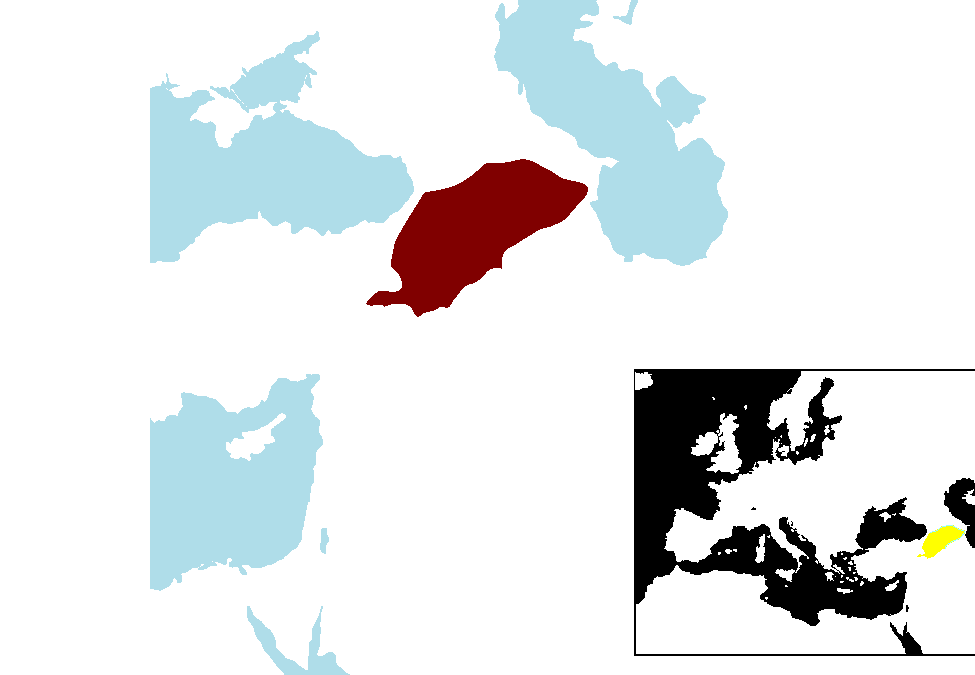
\includegraphics[width=0.25\linewidth, trim=0 0 0 0, clip]{img/unnamed-chunk-15-1} 

\caption{Roman province of Armenia (ca 117 AD).}\label{fig:unnamed-chunk-15}
\end{figure}

Transformation of the entire province from the \texttt{EDH} dataset
requires extracting first a list with the province content. Function
\texttt{edhw()} is to obtain available inscriptions per province from
\texttt{EDH} and all data attributes from \texttt{people} variable. The
default outputs are a list and a dataframe for the first and the second
instance of the function.

\begin{Shaded}
\begin{Highlighting}[]
\CommentTok{# people in Armenia}
\KeywordTok{edhw}\NormalTok{(}\DataTypeTok{province=}\StringTok{"Arm"}\NormalTok{) }\OperatorTok{|}\ErrorTok{>}\StringTok{ }
\StringTok{  }\KeywordTok{edhw}\NormalTok{(}\DataTypeTok{vars=}\StringTok{"people"}\NormalTok{)}
\end{Highlighting}
\end{Shaded}

\begin{verbatim}
        id         age: years        cognomen gender
1 HD015521               <NA> Nerva+ Traianus   male
2 HD015524 data not available        Cre(---)   male
3 HD015524               <NA>           [---]   male
                                 name     nomen person_id praenomen             status
1 div[i] Nervae f[il. N]erva Traianus      <NA>         1      <NA>               <NA>
2                        C. Val. Cre. Valerius*         1        C. military personnel
3                               [---]     [---]         2       [-] military personnel
\end{verbatim}

People attribute variables in inscriptions for \texttt{Armenia} are
\texttt{age:\ years}, \texttt{cognomen}, \texttt{gender}, \texttt{name},
\texttt{nomen}, \texttt{person\_id}, \texttt{praenomen}, and,
\texttt{status}, but any inscription with \texttt{tribus} or
\texttt{origo} as in the case of other provinces.

For \texttt{Armenia}, two inscriptions have people variables and all
people scripted are \texttt{male}, where record \texttt{HD015524} spans
two rows because there are two persons where one have \texttt{nomen},
\texttt{cognomen}, and \texttt{name} ineligible.

\hypertarget{datasets-for-cartographical-maps}{%
\subsubsection{Datasets for cartographical
maps}\label{datasets-for-cartographical-maps}}

The plotting of the Roman province in the previous section requires
other datasets. Apart from \texttt{"rp"}. In \texttt{"sdam"}, there are
other three datasets invoked for plotting cartographical maps related to
the Roman Empire and the Mediterranean basin, which are \texttt{"rpmp"},
\texttt{"rpmcd"}, and \texttt{"retn"}.

Function \texttt{plot.map()} calls dataset \texttt{"rpmp"} for the
shapes and colours in the plotting of the cartographical maps of
different regions of the Roman Empire. For the caption and province
dates with this function shapes and colours are in dataset
\texttt{"rpmcd"}.

\begin{itemize}
\tightlist
\item
  Dataset \texttt{"retn"} bears the shapes of places and routes of an
  ancient transportation system in the Mediterranean region and
  political divisions of the Roman Empire. It also has it contours and
  parts of the European continent.
\end{itemize}

\begin{Shaded}
\begin{Highlighting}[]
\CommentTok{# land contour around Mediterranean}
\KeywordTok{plot.map}\NormalTok{(}\DataTypeTok{type=}\StringTok{"plain"}\NormalTok{)}
\end{Highlighting}
\end{Shaded}

{\centering
\includegraphics[width=9cm, trim=0 0 0 0, clip]{img/unnamed-chunk-18-1} 
%\includegraphics{Intro_files/figure-latex/unnamed-chunk-18-1.pdf}
}

\begin{Shaded}
\begin{Highlighting}[]
\CommentTok{# display settlements and shipping routes}
\KeywordTok{plot.map}\NormalTok{(}\DataTypeTok{type=}\StringTok{"plain"}\NormalTok{, }\DataTypeTok{settl=}\OtherTok{TRUE}\NormalTok{, }\DataTypeTok{shipr=}\OtherTok{TRUE}\NormalTok{)}
\end{Highlighting}
\end{Shaded}

Vignette \href{../doc/Maps.html}{Cartographical maps and networks} has
more about transportation networks in the ancient Mediterranean.

\hypertarget{datasets-with-dates}{%
\subsubsection{Datasets with dates}\label{datasets-with-dates}}

There are built-in datasets in \texttt{"sdam"} related to dates as well
that are either displayed in a cartographical map or used for other
computations.

\begin{itemize}
\tightlist
\item
  Dataset \texttt{"rpd"} that has dates for provinces from the
  \texttt{EDH} dataset. It serves for performing a restricted imputation
  on data subsets in \texttt{EDH} or in another dataset.
\end{itemize}

\begin{Shaded}
\begin{Highlighting}[]
\CommentTok{# dates from EDH}
\KeywordTok{data}\NormalTok{(}\StringTok{"rpd"}\NormalTok{)}

\CommentTok{# three provinces in object structure}
\KeywordTok{str}\NormalTok{(rpd[}\DecValTok{1}\OperatorTok{:}\DecValTok{3}\NormalTok{])}
\end{Highlighting}
\end{Shaded}

\begin{verbatim}
List of 3
 $ Ach: 'HD001917' num [1:4] 105 -190 571 761
 $ Aeg: 'HD000741' num [1:4] 144 -71 500 571
 $ Aem: 'HD000010' num [1:4] 121 -201 771 972
\end{verbatim}

From this set of three Roman provinces in the \texttt{EDH}, the longest
timespan is for \texttt{Aem}, and on average \texttt{Ach} has the oldest
incriptions, while \texttt{Aeg} has incriptions with the newest dates.

\begin{itemize}
\tightlist
\item
  Dataset \texttt{"rpcp"} with chronological periods for regions with
  early and later Roman influence per province.
\end{itemize}

\begin{Shaded}
\begin{Highlighting}[]
\CommentTok{# periods for Roman provinces}
\KeywordTok{data}\NormalTok{(}\StringTok{"rpcp"}\NormalTok{)}

\CommentTok{# object structure}
\KeywordTok{str}\NormalTok{(rpcp)}
\end{Highlighting}
\end{Shaded}

\begin{verbatim}
List of 2
 $ Early:'data.frame':  45 obs. of  3 variables:
  ..$ Province: chr [1:45] "Italia (Final Consolidation)" "Sicilia" "Sardinia & Corsica" "Hispania Ulterior (Later Baetica)" ...
  ..$ EarInf  : num [1:45] -509 -241 -238 -206 -206 -206 -202 -202 -188 -188 ...
  ..$ OffPrv  : num [1:45] -272 -241 -238 -197 -197 -197 -146 -81 43 -133 ...
 $ Late :'data.frame':  45 obs. of  3 variables:
  ..$ Province: Factor w/ 45 levels "Achaea","Aegyptus",..: 30 43 42 27 28 26 3 23 32 9 ...
  ..$ LateInf : num [1:45] 476 436 436 409 409 ...
  ..$ Fall    : num [1:45] 476 436 436 409 409 409 409 418 1400 1500 ...
\end{verbatim}

The early and later Roman influence in the 45 ancient provinces and
regions are timespans with a \emph{terminus ante quem} and a
\emph{terminus post quem}.

Vignette \href{../doc/Dates.html}{Dates and missing dating data} has the
visualisation of these and other dates.

\hypertarget{external-data}{%
\subsubsection{External data}\label{external-data}}

Apart from the built-in datasets, it is attached as external data the
semi-colon separated file \texttt{StraussShipwrecks.csv} with the
Shipwrecks dataset for performing analyses: Reference and documentation
in

Strauss, J. (2013). \emph{Shipwrecks Database}. Version 1.0. Accessed
(07-12-2021) from
oxrep.classics.ox.ac.uk/databases/shipwrecks\_database/

Built from Parker, A.J. \emph{Ancient Shipwrecks of the Mediterranean
and the Roman Provinces} (Oxford: BAR International Series 580, 1992)

Details about the access to the database are in:

\begin{itemize}
\item
  \href{https://htmlpreview.github.io/?https://github.com/sdam-au/R_code/blob/master/HTML/Shipwrecks\%20Network\%20in\%20the\%20Mediterranean\%20Basin.html}{Shipwrecks
  network in the Mediterranean Basin (23-June-2022)}
\item
  Vignettes \href{../doc/Dates.html}{Dates and missing dating data} and
  \href{../doc/Maps.html}{Cartographical maps and networks} also use the
  Shipwrecks dataset.
\end{itemize}


\end{document}
